\section{Experiments}

\subsection{Datasets}
We use four public industrial anomaly benchmarks (MVTec-AD~\cite{Bergmann_2019_CVPR}, VisA~\cite{VisA}, MPDD~\cite{mpdd}, and Real-IAD~\cite{wang2024realiadrealworldmultiviewdataset}), plus VisA-D\&R~\cite{xu2025towards} for defect reasoning, covering the three tasks of Sec.~\ref{sec:prelims} and defect reasoning/analysis. Additional details are in Appendix.

\subsection{Experimental Settings}
We build GenAU on LLaVA-OneVision~\cite{li2025llavaonevision}, which pairs a Qwen2 language backbone with a frozen SigLIP-so400m-patch14-384 vision encoder, and report results at the 0.5B and 7B scales. Following prior zero-shot protocols~\cite{sadikaj2025multiadsdefectawaresupervisionmultitype, chen2023zero, zhou2024anomalyclip}, GenAU is fine-tuned on the test split of MVTec-AD (its only split carrying anomaly masks and defect-type labels, the train split being normal-only) and evaluated, without retraining, on VisA, MPDD, and Real-IAD; MVTec-AD is thus purely the source domain and is disjoint from every evaluation target.
High-resolution inputs use AnyRes (\texttt{anyres\_max\_9}, up to a $6\times6$ grid of $384$-px tiles); the segmentation readout reassembles the tiles into a high-resolution feature grid, fused with the global view ($\beta=0.25$, temperature $20$) using patch features from vision-encoder layers $6,12,18,27$. We adapt only LoRA~\cite{hu2021loralowrankadaptationlarge} ($r=16$, $\alpha=32$) on the LLM, the token embeddings and LM head (to add the two segmentation tokens), the cross-modal projector, and the per-stage projectors and decoder layer-norms; only the encoder stays frozen. For half of the $1{,}725$ training images the segmentation exchange is part of a multi-turn reasoning conversation~\cite{xu2025towards}; each image appears once, so training keeps $53$ steps (Appendix~\ref{app:data}). The segmentation loss combines focal, Tversky ($\alpha=0.3$, $\beta=0.7$), and Dice, with $\lambda=1$ (Eq.~\ref{eq:overall-loss}) and no separate image-level loss; the image score is the fused score $s_{\mathrm{fused}}$ of Sec.~\ref{subsec:seg}. We train one epoch at effective batch size $32$ ($lr=10^{-4}$ cosine, warmup $0.03$, no weight decay; $8$ GPUs, ZeRO-3). All tasks use one checkpoint per scale, with no weight changes between tasks. Further details, including the multi-type prompt and parser, are in Appendix.

\subsection{Evaluation Metrics}
We report image-level AUROC and AP for detection; pixel-level AUROC and AUPRO for segmentation; weighted Precision/Recall/F1 for multi-type detection (to handle class imbalance); and, for reasoning, the VisA-D\&R GPT-Score~\cite{xu2025towards}, where GPT-4o rates each response $1$--$10$ for low-level (perception) and complex (causal-reasoning) questions separately (full definitions in Appendix).

\subsection{Baselines}
All baselines, like GenAU, access only the query image at test time: no reference, support, or exemplar images. As \emph{CLIP-based} zero-shot detectors and segmenters we compare against CLIP, CLIP-AC~\cite{radford2021}, WinCLIP~\cite{jeong2023winclip}, APRIL-GAN~\cite{chen2023zero}, CoOp~\cite{CoOp}, CoCoOp~\cite{zhou2022conditionalpromptlearningvisionlanguage}, AnomalyCLIP~\cite{zhou2024anomalyclip}, AdaCLIP~\cite{Cao_2024}, FiLo~\cite{gu2024filozeroshotanomalydetection}, and MultiADS together with its variant MultiADS-F~\cite{sadikaj2025multiadsdefectawaresupervisionmultitype}, the only CLIP-based baseline that additionally performs multi-type detection. For the multi-type and reasoning tasks we further compare against \emph{vision--language} baselines: the anomaly-reasoning specialist Anomaly-OV~\cite{xu2025towards} and our LLaVA-OneVision~\cite{li2025llavaonevision} backbone, both at the $0.5$B and $7$B scales. Methods without public implementations (e.g., SimCLIP~\cite{simclip}) are excluded for reproducible comparison.

\subsection{Results}
Next, we present and discuss results for binary anomaly detection and segmentation under distribution shift, multi-type zero-shot anomaly detection, and defect reasoning, the four tasks GenAU addresses within a single model.
\subsubsection{Binary Detection and Segmentation under Distribution
Shift}
Table~\ref{tab:binary} reports the performance of GenAU on VisA, MPDD, and Real-IAD, compared with state-of-the-art CLIP-based methods. Pixel-level metrics (AUROC, AUPRO) and image-level metrics (AUROC, AP) are reported.

On VisA, the 7B model achieves the best image-level AUROC ($90.1\%$) among the methods in Table~\ref{tab:binary}; the VLM reasoning specialist Anomaly-OV-7B reports a VisA image-AUROC of $88.9\%$ but is trained under an instruction-tuning rather than our cross-dataset protocol and produces no segmentation, so we note it here only for context. On MPDD, GenAU-7B attains the highest pixel-level AUROC and AUPRO ($96.7\%$, $89.8\%$) and image-level AP ($85.1\%$), while its image-level AUROC ($78.7\%$) stays below MultiADS-F ($79.7\%$), reflecting the logical and large-area anomalies of this dataset. On Real-IAD, it reaches an image-level AUROC of $85.1\%$ and the highest pixel-level AUPRO ($88.2\%$). Its pixel-level scores on VisA, however, remain below the strongest CLIP-based segmenters. The 0.5B variant remains competitive, with the second-best image-level AUROC on VisA and Real-IAD.
Overall, GenAU demonstrates that a single instruction-following VLM can achieve strong binary detection and segmentation performance under distribution shift.
\begin{table}
\setlength{\tabcolsep}{2pt}
\centering
	\caption[Results of GenAU for binary anomaly detection and segmentation under distribution shift]{Zero-shot binary detection and segmentation under distribution shift (\%). \textbf{Bold}/\underline{underline}: best/second best. Baseline numbers are quoted from MultiADS~\cite{sadikaj2025multiadsdefectawaresupervisionmultitype} and FiLo~\cite{gu2024filozeroshotanomalydetection} and are \emph{not} recomputed in our harness.}
	\label{tab:binary}
\begin{tabular}{c|ccccc}
\toprule
\multirow{2}{*}{\textbf{Dataset}} & \multirow{2}{*}{\textbf{Method}}  
& \multicolumn{2}{c}{\textbf{Pixel-Level}} & \multicolumn{2}{c}{\textbf{Image-Level}} \\
\cmidrule{3-6}
& & \textbf{AUROC} & \textbf{AUPRO} & \textbf{AUROC} & \textbf{AP} \\
\midrule
\multirow{13}{*}{VisA}
& CLIP        & 46.6 & 14.8 & 66.4 & 71.5 \\
& CLIP-AC     & 47.8 & 17.3 & 65.0 & 70.1 \\
& CoOp        & 24.2 & 3.8 & 62.8 & 68.1 \\
& CoCoOp      & 93.6 & - & 78.1 & - \\
& WinCLIP     & 79.6 & 56.8 & 78.1 & 81.2 \\
& APRIL-GAN   & 94.2 & 86.8 & 78.0 & 81.4 \\
& AnomalyCLIP  & \underline{95.5} & 87.0 & 82.1 & 85.4 \\
& AdaCLIP     & 95.0 & - & 75.4 & 79.3 \\
& FiLo     & \textbf{95.9} & - & 83.9 & - \\
& MultiADS   & 95.0 & \textbf{89.7} & 83.6 & 86.9\\
& MultiADS-F & 94.5 & 87.4 & 82.5 & 86.5 \\
\cmidrule(lr){2-6}
% 2026-10-17: GenAU rows = halfmix checkpoints (hires-tversky{,-05b}-halfmix-proj), runs halfmix-{7b,05b}-<ds>-fair,
% fused with their own MVTec calibration (evaluation/fusion_calib_halfmix{,05b}_ens8.json).
&  GenAU-0.5b &      95.0 & \underline{88.2} & \underline{89.2} & \underline{90.9} \\
&  GenAU-7b &      94.4 & 87.4 & \textbf{90.1} & \textbf{91.8} \\
\midrule
\multirow{12}{*}{MPDD}
& CLIP        & 62.1 & 33.0 & 54.3 & 65.4 \\
& CLIP-AC     & 58.7 & 29.1 & 56.2 & 66.0 \\
& CoOp        & 15.4 & 2.3  & 55.1 & 64.2 \\
& CoCoOp      & 95.2 & - & 61.0 & - \\
& WinCLIP      & 76.4 & 48.9 & 63.6 & 69.9 \\
& APRIL-GAN    & 94.1 & 83.2 & 73.0 & 80.2 \\
& AnomalyCLIP  & 96.5 & 88.7 & 77.0 & 82.0 \\
& AdaCLIP      & 96.3 & - & 66.3 & 75.0 \\
& MultiADS   & 95.8 & \underline{89.7} &  78.3 & 78.4 \\
& MultiADS-F & 96.3 & 89.5 & \textbf{79.7} & 80.5 \\
\cmidrule(lr){2-6}
& GenAU-0.5b &   \underline{96.6} & 88.1 & 76.2 & \underline{82.6} \\
& GenAU-7b &       \textbf{96.7} & \textbf{89.8} & \underline{78.7} & \textbf{85.1} \\
\midrule
\multirow{8}{*}{Real-IAD} 
& WinCLIP      & 87.1 & 59.9 & 75.0 & 72.3 \\
& APRIL-GAN    & 96.0 & 86.8 & 75.7 & 73.5 \\
& AnomalyCLIP  & 96.2 & 85.7 & 78.4 & 76.7 \\
& AdaCLIP      & 95.3 & - & 70.1 & 68.5 \\
& MultiADS   & \textbf{96.6} & 87.1 & 78.7 & 79.1\\
& MultiADS-F   &  \underline{96.3} & \underline{87.2} & 78.2 & 78.5 \\
\cmidrule(lr){2-6}
& GenAU-0.5b &        89.5 & 75.1 & \underline{84.3} & \underline{84.9}\\
& GenAU-7b &        \underline{96.3} & \textbf{88.2} & \textbf{85.1} & \textbf{85.4}\\
\bottomrule
\end{tabular}
\end{table}
Qualitative results of GenAU and the best overall performer, MultiADS, are shown in Figure~\ref{fig:visa-visual-good} (and, for a failure case, Figure~\ref{fig:visa-visual-bad}). GenAU accurately segments visually salient defects such as \textit{hole}, \textit{broken}, and \textit{crack}, and produces cleaner, lower-noise segmentation maps than MultiADS. However, global-context or logic-dependent defects such as \textit{missing} components remain challenging. For these cases, similarity maps are low-confidence, often resulting in incomplete localization or misclassification of normal regions for both models (Figure~\ref{fig:visa-visual-bad}).

\begin{figure}[h]
  \centering
  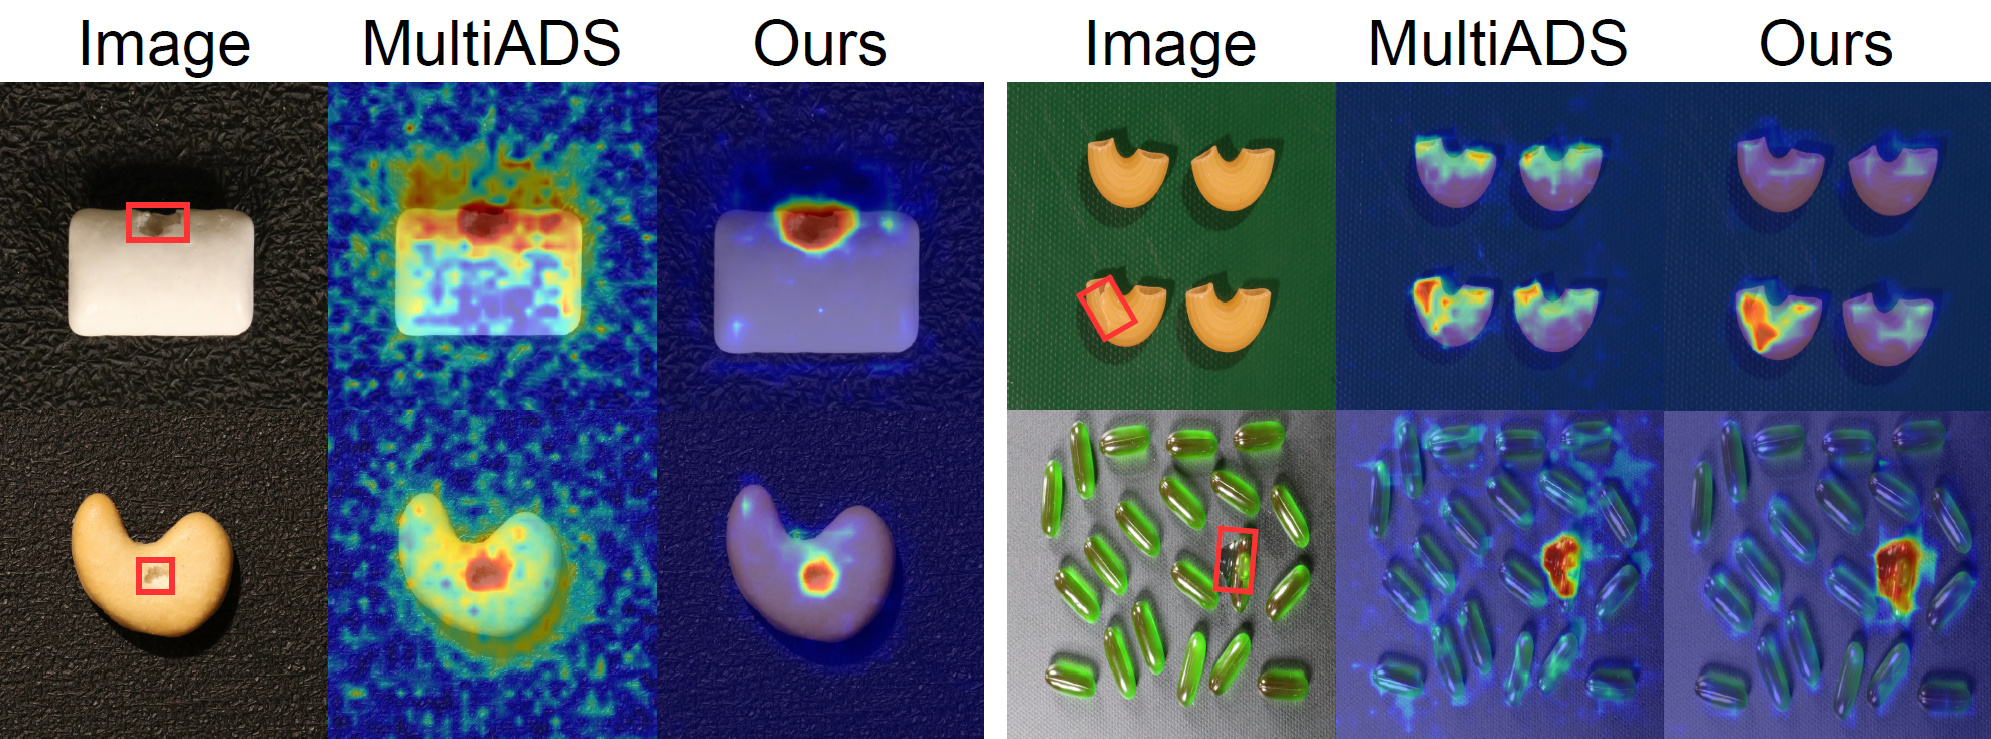
\includegraphics[width=1.0\columnwidth]{imgs/Visa-visual.jpg}
  \caption{Visualization of anomaly segmentation under distribution shift from VisA. Results are compared with MultiADS.}
   \label{fig:visa-visual-good}
\end{figure}

\textbf{Ablation Studies}.\label{sec:ablations}
Replacing decoder-conditioned anchors with randomly initialized, trainable constant queries lowers VisA pixel-AUPRO from $88.7$ to $87.4$ (Table~\ref{tab:ablations_main}). Under matched inference, decoder anchors improve pixel-AUPRO by $1.28$ points on VisA and $0.19$ on MPDD, but trail by $1.78$ on Real-IAD. Across three training seeds, the mean differences are $+4.40$, $-0.47$, and $-0.68$ points, respectively: the localization benefit is dataset-dependent, not universal. Both arms produce maps for every image, using the appended-token fallback when needed.
Table~\ref{tab:ablations_main} varies one factor at a time on VisA. Removing the LM fusion (\emph{map-max only}) lowers image-AUROC by $5.6$ points ($90.1\!\rightarrow\!84.5$); fusing the log-odds of only the single question an image is asked recovers $2.2$ of them ($86.7$), so averaging over phrasings supplies most of the gain. The VLM prior is useful by itself: untrained LLaVA-OneVision, asked the same eight questions, reaches $87.0$ image-AUROC from its yes/no log-odds alone, above every CLIP baseline in Table~\ref{tab:binary} (on Real-IAD, $84.4$ versus $78.7$); fine-tuning raises this term to $89.2$. Training on segmentation alone, at the same $53$ steps, adds $1.8$ pixel-AUPRO but no detection, and segmentation-only checkpoints answer complex VisA-D\&R questions poorly (SBERT similarity $0.576$ versus $0.664$; Appendix~\ref{app:eval}). Giving every training image a reasoning conversation (\emph{full reasoning mix}) instead doubles the optimization steps and costs $3.5$ image-AUROC and $2.9$ pixel-AUPRO, so our default embeds reasoning in half of the samples at an unchanged budget. Freezing the LLM decoder -- keeping the adapter attached but untrained -- leaves detection and localization nearly unchanged ($90.0$ image-AUROC, $88.0$ AUPRO), but the frozen decoder rarely emits the segmentation tokens on its own (they are appended for $1{,}984$ of $2{,}162$ VisA images): adapting the decoder lets the model request segmentation itself, rather than improving the readout or the decision. The ablation studies of hyper-parameters are in Appendix.

\begin{table}
\small
\centering
\setlength{\tabcolsep}{3pt}
\caption{GenAU-7B ablations on VisA (\%). The shaded row is our default; each indented row changes one factor of the nearest less-indented row above it. $^\ast$Also halves the text-loss weight. Image columns use the fused score of Table~\ref{tab:binary}.}
\label{tab:ablations_main}
\begin{tabular}{@{}l|cc|cc@{}}
\toprule
 & \multicolumn{2}{c|}{\textbf{Pixel}} & \multicolumn{2}{c}{\textbf{Image}} \\
\cmidrule(lr){2-3}\cmidrule(lr){4-5}
 & AUROC & AUPRO & AUROC & AP \\
\midrule
% 2026-10-07: every row re-evaluated with the appended-token inference step (SEG_FORCE_ANCHORS=1,
% evaluation_summary_*-fair). The comments below describe the earlier, pre-fix values.
% 2026-10-10: image columns = fused score with the 8-phrasing LM term (evaluation/fusion_calib_tversky_ens8.json,
% w=1), from evaluation/lm_decision/<tag>-visa_s*.npz + per_sample_<run>.jsonl; same frozen calibration on every row.
% 2026-10-17 (halfmix default). Default + w/o fusion + single-question: halfmix-7b-visa-fair with its own calibration
% (fusion_calib_halfmix_ens8.json; single question: assigned-question log-odds, MVTec-standardized, w=0.5).
% segmentation only = noreason-proj (trainable projector); frozen projector = the earlier default hires-tversky-1layer-1ep-bs32.
% These rows use fusion_calib_tversky_ens8.json. frozen LLM = noreason-proj-lm05-nolora-s42 (projector trained, LM-loss weight 0.5).
% LQA image columns: 8-phrasing dump job 5190332 (single-question score was 86.7 / 89.1).
\rowcolor{gray!20}
GenAU-7B (default) & 94.4 & 87.4 & 90.1 & 91.8 \\
\midrule
\quad w/o LM fusion & 94.4 & 87.4 & 84.5 & 87.6 \\
\quad single-question LM term & 94.4 & 87.4 & 86.7 & 89.2 \\
\quad segmentation only & 95.6 & 89.2 & 89.9 & 91.5 \\
\qquad frozen LLM$^\ast$ & 95.2 & 88.0 & 90.0 & 91.7 \\
\qquad frozen projector & 95.1 & 88.7 & 90.5 & 91.9 \\
\qquad\quad learned-query anchors & 94.3 & 87.4 & 89.0 & 90.9 \\
\qquad\quad full reasoning mix & 95.1 & 85.8 & 87.0 & 89.6 \\
\midrule
% Base LLaVA-OV-7B, no anomaly training: mean yes/no log-odds over the 8 phrasings only (evaluation/lm_decision/base-visa_s*.npz).
untrained LLaVA-OV, LM only & -- & -- & 87.0 & 89.4 \\
\bottomrule
\end{tabular}
\end{table}


\subsubsection{Zero-Shot Multi-Type Detection}
We evaluate candidate-list-conditioned defect-type classification on known-anomalous images of VisA and MPDD (Table~\ref{tab:multytype_zero_shot_detection_performance}). The prompt supplies the target object's possible coarse defect labels and asks for one label; compound defects may form a \emph{combined} class, rather than being decoded as multiple independent labels. This is conditional type recognition, not joint normal/anomalous and multi-label prediction. The mapped evaluation subsets contain $916$ VisA and $282$ MPDD images; unmapped labels are excluded (Appendix~\ref{app:eval}).
GenAU-7B, the checkpoint of Table~\ref{tab:binary}, obtains weighted F1 of $33.4\%$ and $89.5\%$, respectively, the highest values in this table. Three of the six MPDD objects have a single candidate label, so an oracle predicting each object's most frequent label already reaches $76.0\%$ there ($31.4\%$ on VisA). Anomaly-OV-0.5B/7B are our MVTec-trained reproductions with a two-turn detect-then-classify prompt. MultiADS, designed for multi-type segmentation, is converted to detection by thresholding its per-type channels at $0.5$; its comparison is therefore operating-point-dependent, not evidence of superiority under an optimized threshold. VisA's finer, object-dependent taxonomy remains difficult despite its higher precision.

\begin{table}
\small
\centering
\caption[Conditional defect-type recognition.]{Conditional defect-type recognition on mapped anomalous images (\%). GenAU uses the checkpoints of Table~\ref{tab:binary}; the prompt and scorer exclude normal as an option. \textbf{Bold}: highest reported value per column. Anomaly-OV uses our MVTec-trained two-turn reproductions; MultiADS uses a fixed $0.5$ channel threshold.}
\label{tab:multytype_zero_shot_detection_performance}
\begin{tabular}{@{}llccc@{}}
\toprule
\textbf{Dataset}          & \textbf{Model} & \textbf{Precision} & \textbf{Recall} & \textbf{F1} \\ \midrule
\multirow{5}{*}{VisA}     & MultiADS         & 17.4          & \textbf{57.7} & 18.6          \\
                          & Anomaly-OV-0.5b  & 18.4          & 11.1          & 9.3           \\
                          & Anomaly-OV-7b  & 42.1          & 30.9          & 21.1           \\
                          \cline{2-5}
% 2026-10-17: halfmix checkpoints, runs halfmix-{05b,7b}-{visa,mpdd}-mtype-nn, score_multitype.py --no-normal.
% Segmentation-only checkpoints gave 0.5b 20.3/21.5/16.4, 18.7/30.5/23.2 and 7b 51.3/42.6/37.4, 92.7/87.9/89.2.
                          & GenAU-0.5b         & 31.1 & 20.9          & 13.8 \\
                          & GenAU-7b         & \textbf{52.4} & 38.3          & \textbf{33.4} \\ \midrule
\multirow{5}{*}{MPDD}     & MultiADS         & 34.0          & 51.3          & 32.7          \\
                          & Anomaly-OV-0.5b  & 60.1          & 30.5           & 29.9          \\
                          & Anomaly-OV-7b  & 87.1          & 65.8           & 65.1          \\
                          \cline{2-5}
                          & GenAU-0.5b         & 42.3 & 54.6          & 46.8 \\
                          & GenAU-7b         & \textbf{91.5} & \textbf{89.4} & \textbf{89.5} \\
% \multirow{1}{*}{Real-IAD}  
%                           & GenAU-7b   & 39.1               & 36.6            & 31.3      
\bottomrule
\end{tabular}
\end{table}



\subsubsection{Defect Reasoning and Analysis}
Beyond detecting and localizing defects, GenAU answers open-ended questions about them. We evaluate on VisA-D\&R~\cite{xu2025towards} (low-level perception and complex causal-reasoning questions) against the reasoning specialist Anomaly-OV~\cite{xu2025towards}; here GenAU augments its segmentation training with a reasoning instruction mix, so one model both localizes and explains, whereas Anomaly-OV produces no segmentation.

Table~\ref{tab:reasoning} gives the reported GPT-Scores. The LLaVA-OneVision and Anomaly-OV numbers are taken from~\cite{xu2025towards}, not rejudged alongside GenAU, so these comparisons are indicative rather than controlled. In particular, the $6.43$ versus $6.34$ complex-reasoning scores do not establish a reliable advantage without a shared judge and uncertainty estimates. Textual plausibility or reference agreement also does not establish the correctness of a causal diagnosis.

\begin{table}
\small
\centering
\setlength{\tabcolsep}{6pt}
\caption{Defect reasoning on VisA-D\&R~\cite{xu2025towards}, scored by GPT-4o on a $1$--$10$ scale. VisA-D\&R poses two question categories per image: \emph{Low-level} perception questions, which ask the model to describe the anomaly, and \emph{Complex} causal-reasoning questions about its significance, likely cause, and prevention; we report the GPT-Score separately for each. $^\dagger$LLaVA-OV and Anomaly-OV scores as reported in the Anomaly-OV paper~\cite{xu2025towards}. For this task GenAU augments its segmentation training with a reasoning instruction mix, and is evaluated as a single model that both localizes and explains anomalies.}
\label{tab:reasoning}
% TODO(GPT-Score): the GenAU rows, this caption and the paragraph above still describe the REASONING-MIX checkpoints.
% Replace with the user's GPT-4o scores of evaluation/gpt_score_input/visa-dr_halfmix-{7b,05b}.json (the Table 1 halfmix checkpoints).
\begin{tabular}{@{}lcc@{}}
\toprule
\multirow{2}{*}{\textbf{Model}} & \multicolumn{2}{c}{\textbf{GPT-Score}} \\
\cmidrule(lr){2-3}
 & \textbf{Low-level} & \textbf{Complex} \\
\midrule
LLaVA-OV-0.5B$^\dagger$   & 2.54 & 4.34 \\
LLaVA-OV-7B$^\dagger$     & 3.57 & 5.44 \\
Anomaly-OV-0.5B$^\dagger$ & 3.87 & 5.67 \\
Anomaly-OV-7B$^\dagger$   & 4.26 & 6.34 \\
\cmidrule(lr){1-3}
GenAU-0.5B & 5.01          & 6.13          \\
GenAU-7B   & 5.22 & 6.43 \\
\bottomrule
\end{tabular}
\end{table}

